\documentclass[letterpaper,12pt]{article}
\usepackage[margin=1in]{geometry}
\usepackage{amsmath}
\usepackage{graphicx}
\usepackage{listings}
\usepackage{pdfpages}
\usepackage{tikz}

\pagestyle{empty}
\lstset{basicstyle=\ttfamily\small,breaklines=true,columns=fullflexible}

% Import the original pages without transcribing, cropping, or scaling them.
\newcommand{\handout}[1]{%
  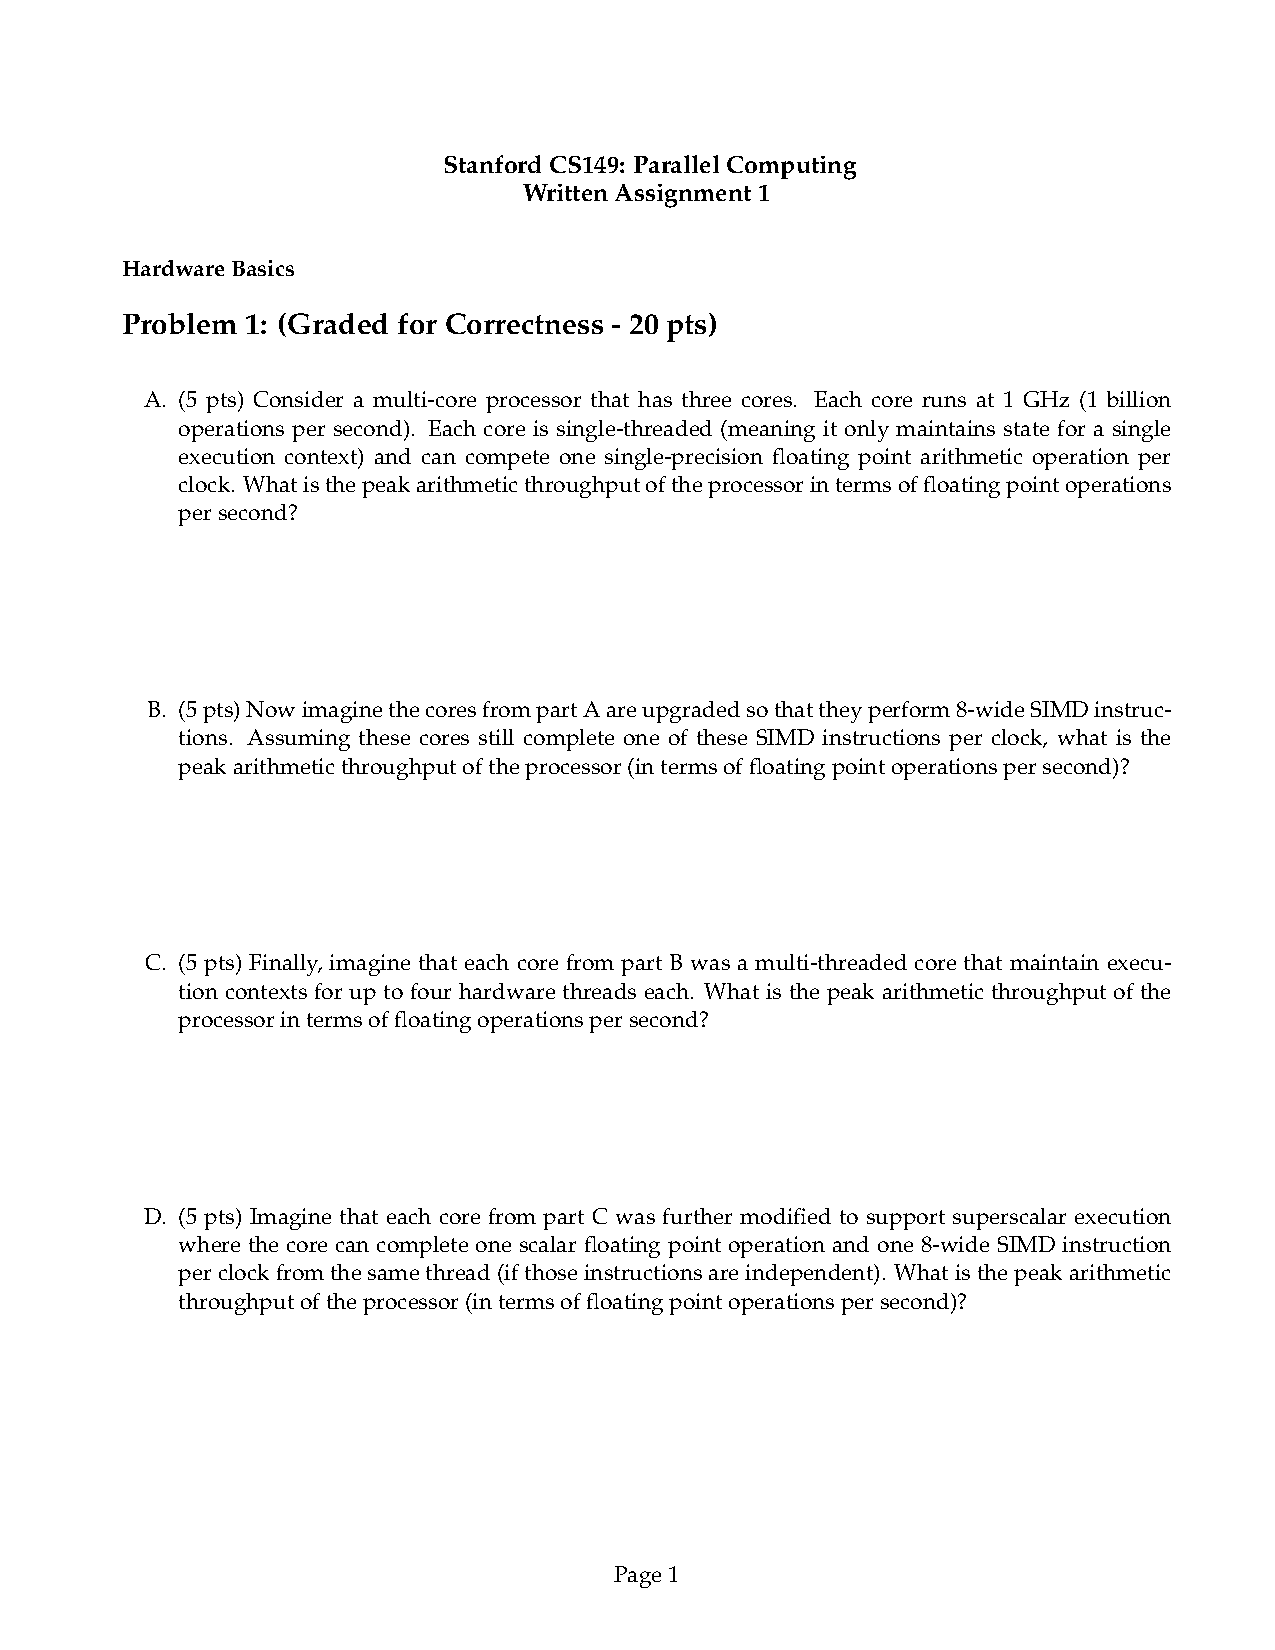
\includepdf[
    pages={#1},
    fitpaper=true,
    noautoscale=true,
    pagecommand={}
  ]{../written_asst1.pdf}
}

% Replace the vertical-space placeholder in each environment with your answer.
% Use lstlisting for code and includegraphics for diagrams when needed.
\newenvironment{answer}{\par}{\par\medskip}

\begin{document}

% Problem 1: original handout pages 1.
\handout{1}
\section*{Problem 1: Answers}
\noindent Original handout: page 1.\par

\subsection*{A}
\begin{answer}
Each core completes one floating-point operation per clock, and
$1\,\mathrm{GHz}=10^9$ clocks per second. With three cores, the peak
arithmetic throughput is
\[
  P_A = 3 \times 10^9 \times 1
      = \boxed{3\times10^9\ \mathrm{FLOP/s}
      = 3\ \mathrm{GFLOP/s}}.
\]
\end{answer}

\subsection*{B}
\begin{answer}
Each 8-wide SIMD instruction performs eight floating-point operations.
Each core still completes one such instruction per clock, so
\[
  P_B = 3 \times 10^9 \times 8
      = \boxed{24\times10^9\ \mathrm{FLOP/s}
      = 24\ \mathrm{GFLOP/s}}.
\]
\end{answer}

\subsection*{C}
\begin{answer}
The four hardware threads per core share the core's execution resources.
Adding execution contexts does not increase the number of SIMD instructions
the core can complete per clock. Hardware multithreading can hide stalls
and help approach peak throughput, but the peak remains unchanged:
\[
  P_C = 3 \times 10^9 \times 8
      = \boxed{24\times10^9\ \mathrm{FLOP/s}
      = 24\ \mathrm{GFLOP/s}}.
\]
\end{answer}

\subsection*{D}
\begin{answer}
Each core can now complete one scalar operation and one independent
8-wide SIMD instruction in the same clock. This gives $1+8=9$
floating-point operations per core per clock. Therefore,
\[
  P_D = 3 \times 10^9 \times (1+8)
      = \boxed{27\times10^9\ \mathrm{FLOP/s}
      = 27\ \mathrm{GFLOP/s}}.
\]
\end{answer}

\clearpage

% Problem 2: original handout pages 2-4.
\handout{2-4}
\section*{Problem 2: Answers}
\noindent Original handout: pages 2--4.\par

\subsection*{A}
\begin{answer}
The graph below is the transitive reduction of the register-ordering
constraints without register renaming. It preserves the same required
instruction ordering while omitting edges already implied by another
directed path. Solid arrows are retained read-after-write (RAW)
dependencies; dashed arrows are retained write-after-read (WAR) constraints.
Instructions 1, 2, and 4 read the initial values of R0 and R1.

\begin{center}
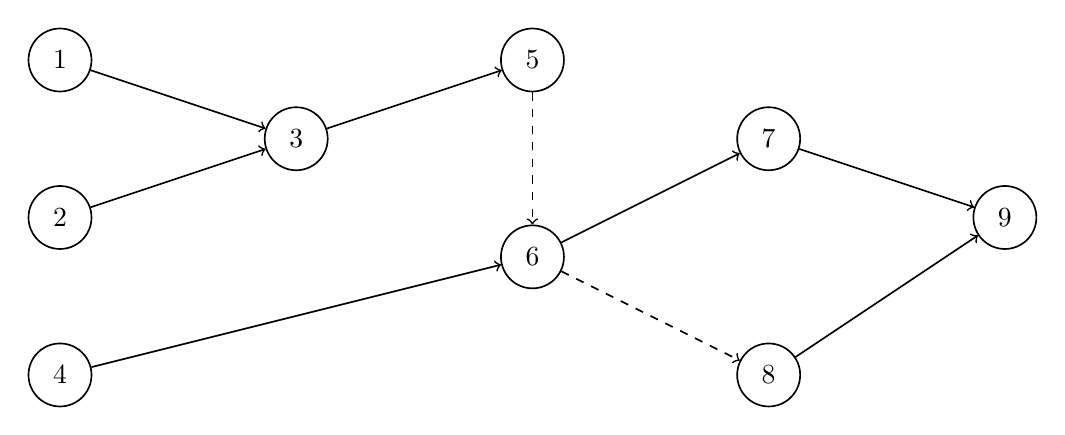
\begin{tikzpicture}[
  ->,semithick,
  instruction/.style={circle,draw,minimum size=8mm,inner sep=1pt}
]
  \node[instruction] (i1) at (0,2) {1};
  \node[instruction] (i2) at (0,0) {2};
  \node[instruction] (i4) at (0,-2) {4};
  \node[instruction] (i3) at (3,1) {3};
  \node[instruction] (i5) at (6,2) {5};
  \node[instruction] (i6) at (6,-0.5) {6};
  \node[instruction] (i7) at (9,1) {7};
  \node[instruction] (i8) at (9,-2) {8};
  \node[instruction] (i9) at (12,0) {9};

  \draw (i1) -- (i3);
  \draw (i2) -- (i3);
  \draw (i3) -- (i5);
  \draw (i4) -- (i6);
  \draw (i6) -- (i7);
  \draw (i7) -- (i9);
  \draw (i8) -- (i9);

  \draw[dashed] (i5) -- (i6);
  \draw[dashed] (i6) -- (i8);
\end{tikzpicture}
\end{center}

For example, $1\to5$ is omitted because the path $1\to3\to5$ already
forces instruction 1 to precede instruction 5. Instruction 5 still reads
the R2 value produced by instruction 1; only the redundant ordering edge
has been removed. The other omitted edges are $3\to6$, $5\to7$, and
$4\to8$, whose ordering is preserved by
\[
  3\to5\to6,\qquad 5\to6\to7,\qquad 4\to6\to8.
\]

Dashed arrows show additional write-after-read (WAR) constraints if the
architectural registers are used without register renaming:
\begin{itemize}
  \item $5\to6$: instruction 5 must read the old R3 before instruction 6
        overwrites it.
  \item $6\to8$: instruction 6 must read the old R4 before instruction 8
        overwrites it.
\end{itemize}
The write-after-write constraints are also implied by the remaining paths.
If register renaming is assumed, the RAW-only graph must be reduced
separately. Simply deleting the dashed arrows from this already reduced
graph would lose paths that currently enforce required RAW ordering.
\end{answer}

\clearpage
\subsection*{B}
\begin{answer}
An optimal schedule is shown below. Entries list the instructions that
\emph{start} in that clock; a dash means no new instruction starts.

\begin{center}
\begin{tabular}{c|*{10}{c}}
  Clock & 1 & 2 & 3 & 4 & 5 & 6 & 7 & 8 & 9 & 10 \\
  \hline
  Start & $2,4,5$ & $1$ & $3,7$ & -- & $6$ & -- & $8,9$ & -- & $10$ & --
\end{tabular}
\end{center}

The three instructions started in clock 1 are all MULs. The ADD instruction 1
starts alone in clock 2, while those MULs are finishing. Thus instruction 3
can start in clock 3: instruction 2 is ready after two clocks, and
instruction 1 is ready after one clock. Instruction 6 starts in clock 5,
instructions 8 and 9 start in clock 7, and instruction 10 starts in clock 9.

Instruction 10 has a two-clock latency, so it executes during clocks 9
and 10. The entire stream therefore finishes at the end of clock 10:
\[
  \boxed{T_{\min}=10\text{ clocks}}.
\]

To prove optimality, consider the dependency chain
\[
  2\longrightarrow3\longrightarrow6\longrightarrow8\longrightarrow10.
\]
All five instructions are MULs, each with latency two clocks, giving a
lower bound of $5\times2=10$ clocks. The schedule attains this bound,
so no legal schedule can finish earlier. The last instruction starts
in clock 9, but completion requires clock 10 as well.
\end{answer}

\subsection*{C}
\begin{answer}
No. The available instruction-level parallelism (ILP) and the critical
dependency chain limit this instruction stream. A five-way processor
still cannot shorten the five-MUL chain, whose latency is 10 clocks.

The three-way schedule in part B already achieves that lower bound.
It starts all three independent MUL roots, instructions 2, 4, and 5,
together, while ADD instruction 1 must start alone under the stated rule.
Increasing the issue width to five therefore leaves the minimum execution
time at $\boxed{10\text{ clocks}}$ and provides no performance improvement
for this stream.
\end{answer}

\clearpage

% Problem 3: original handout pages 5.
\handout{5}
\section*{Problem 3: Answers}
\noindent Original handout: page 5.\par

\subsection*{A}
\begin{answer}
For each stage, its capacity is the number of graders divided by the time
one grader takes to process an exam:

\begin{center}
\begin{tabular}{c|c|c|c}
  Stage & Graders & Time per exam per grader & Capacity (exams/min) \\
  \hline
  Q1 & 2 & 3 min & $2/3$ \\
  Q2 & 3 & 1 min & $3$ \\
  Each of Q3--Q7 & 1 & 1 min & $1$
\end{tabular}
\end{center}

The steady-state throughput is limited by the stage with the lowest
capacity. Therefore,
\[
  R = \min\left(\frac{2}{3},3,1,1,1,1,1\right)
    = \boxed{\frac{2}{3}\text{ exams per minute}}.
\]
Q1 is the bottleneck. Once the pipeline is filled, the average completion
rate is one exam every $3/2=1.5$ minutes; all later stages have sufficient
capacity to sustain this rate.
\end{answer}

\subsection*{B}
\begin{answer}
Assuming the exam does not wait between stages, its latency is the sum
of its processing times for all seven questions:
\[
  L = 3 + \underbrace{1+1+1+1+1+1}_{\text{Q2 through Q7}}
    = \boxed{9\text{ minutes}}.
\]
The parallel graders work on different exams. A particular exam still
needs 3 minutes for Q1 and 1 minute for each subsequent question.

This is the processing latency; an exam's actual elapsed latency is
$9$ minutes plus any queueing delay. For example, if both Q1 graders
start together, their exams reach Q3 together. With the downstream
pipeline initially empty, one exam can finish in 9 minutes while the
other waits one minute at Q3 and finishes in 10 minutes. Picking up work
immediately when a grader is free eliminates avoidable idle time, but
does not eliminate waiting for a busy grader.
\end{answer}

\clearpage

% Problem 4: original handout pages 6.
\handout{6}
\section*{Problem 4: Answers}
\noindent Original handout: page 6.\par

\subsection*{A}
\begin{answer}
Each cache line holds one float. With $N=10^9$, the input and output arrays
occupy about $8\times10^9$ bytes in total, far exceeding the 16 MB cache.
Under the streaming-cache model, an input value is evicted before the next
outer-loop pass reuses it, so we treat the loads as cache misses.

Each thread alternates between waiting 50 clocks for a load and executing
10 dependent floating-point operations. Its load/compute period is therefore
$50+10=60$ clocks. Infinite memory bandwidth allows the two threads' memory
requests to overlap. One repeating schedule after startup is:

\begin{center}
\begin{tabular}{c|l}
  Clock interval & Core activity \\
  \hline
  $[0,10)$ & Thread 0 executes its 10 multiplies \\
  $[10,20)$ & Thread 1 executes its 10 multiplies \\
  $[20,60)$ & Both threads wait for memory; the core is idle
\end{tabular}
\end{center}

Thread 0 issues its next load at time 10, ready at time 60; thread 1 issues
its next load at time 20, ready at time 70. The same pattern then repeats
60 clocks later. Thus, 20 of every 60 clocks perform floating-point work:
\[
  U = \frac{2\times10}{50+10}
    = \boxed{\frac{1}{3}\approx33.3\%}.
\]
This uses the simplified blocking-load model and ignores unspecified
loop-control, load-issue, and thread-switch overheads.
\end{answer}

\clearpage
\subsection*{B}
\begin{answer}
\textbf{Choose the 25\% increase in clock rate.}
For $N=10^6$, the combined footprint of the two float arrays is
\[
  2\times10^6\times4 = 8\times10^6\text{ bytes},
\]
which fits in the 16 MB cache, even when both input and output are cached.
The two threads work on disjoint halves of these arrays; they do not
require separate copies.

After the initial pass brings the data into cache, later passes reuse
cached input values. Cache-hit latency and memory-write latency are both
zero in the model, so execution becomes compute-bound. The 1000 outer-loop
passes make this warm-cache behavior dominate the total execution time.

With one floating-point operation per clock, increasing the frequency
from $f$ to $1.25f$ gives approximately $1.25\times$ steady-state throughput:
\[
  \frac{T_{\mathrm{new}}}{T_{\mathrm{old}}}
  \approx\frac{1}{1.25}=0.8.
\]
Reducing the miss latency from 50 to 20 clocks mainly improves the initial
cache fill, with little benefit for the subsequent cache-hit passes.
The higher clock rate therefore gives the larger overall speedup.
\end{answer}

\clearpage

% Problem 5: original handout pages 7-8.
\handout{7-8}
\section*{Problem 5: Answers}
\noindent Original handout: pages 7--8.\par

\subsection*{A}
\begin{answer}
Each row is processed in four groups of four adjacent pixels. An all-white
group executes only \texttt{foo}, costing 1 clock; an all-dark group
executes only \texttt{bar}, costing 10 clocks. A mixed group executes both
branches under different lane masks, costing $1+10=11$ clocks.

Number rows within one repeating block from 0 to 12. Each row has four
consecutive dark pixels, starting in column equal to its row number.
Rows 0, 4, 8, and 12 have one all-dark group and three all-white groups.
Each of the other nine rows has two mixed groups and two all-white groups.
Thus, one 13-row block contains:

\begin{center}
\begin{tabular}{c|c|c|c}
  Group type & Number of groups & Clocks per group & Total clocks \\
  \hline
  All white & $4\times3+9\times2=30$ & 1 & 30 \\
  All dark & 4 & 10 & 40 \\
  Mixed & $9\times2=18$ & 11 & 198
\end{tabular}
\end{center}

Each block therefore takes $30+40+198=268$ clocks. Since $N$ is divisible
by 13, the complete image takes
\[
  T(N)=\frac{N}{13}\left(30\times1+4\times10+18\times11\right)
      =\boxed{\frac{268N}{13}\text{ clocks}}.
\]
This ordinary ISPC invocation runs on one calling thread; its four
program instances are SIMD lanes. The eight supported hardware thread
contexts do not automatically create eight parallel invocations or
divide this execution time by eight.
\end{answer}

\subsection*{B}
\begin{answer}
SIMD utilization is the number of useful active-lane clocks divided by
the total available lane clocks. In each 13-row block there are
$13\times4=52$ dark pixels and $13\times12=156$ white pixels. A white
pixel needs one arithmetic clock, while a dark pixel needs ten, giving
\[
  W=156\times1+52\times10=676
\]
useful active-lane clocks. The four-wide SIMD unit provides
$4\times268=1072$ available lane clocks over the same block. Therefore,
\[
  U=\frac{676}{4\times268}
   =\frac{169}{268}
   \approx\boxed{63.06\%}.
\]
Both counts scale by $N/13$, so the utilization is independent of $N$.
This weights each group's utilization by its execution time, rather
than taking an unweighted average over the groups.
\end{answer}

\clearpage

% Practice Problem 1: original handout pages 9-11.
\handout{9-11}
\section*{Practice Problem 1: Answers}
\noindent Original handout: pages 9--11.\par

\subsection*{A}
\begin{answer}
  \vspace{2cm}
\end{answer}

\subsection*{B}
\begin{answer}
  \vspace{2cm}
\end{answer}

\clearpage

% Practice Problem 2: original handout pages 12-14.
\handout{12-14}
\section*{Practice Problem 2: Answers}
\noindent Original handout: pages 12--14.\par

\subsection*{A}
\begin{answer}
  \vspace{2cm}
\end{answer}

\subsection*{B}
\begin{answer}
  \vspace{2cm}
\end{answer}

\subsection*{C}
\begin{answer}
  \vspace{2cm}
\end{answer}

\subsection*{D}
\begin{answer}
  \vspace{2cm}
\end{answer}

\clearpage

% Practice Problem 3: original handout pages 15-18.
\handout{15-18}
\section*{Practice Problem 3: Answers}
\noindent Original handout: pages 15--18.\par

\subsection*{A}
\begin{answer}
  \vspace{2cm}
\end{answer}

\subsection*{B}
\begin{answer}
  \vspace{2cm}
\end{answer}

\subsection*{C}
\begin{answer}
  \vspace{2cm}
\end{answer}

\subsection*{D}
\begin{answer}
  \vspace{2cm}
\end{answer}

\subsection*{E}
\begin{answer}
  \vspace{2cm}
\end{answer}

\clearpage

% Practice Problem 4: original handout pages 19-22.
\handout{19-22}
\section*{Practice Problem 4: Answers}
\noindent Original handout: pages 19--22.\par

\subsection*{A}
\begin{answer}
  \vspace{2cm}
\end{answer}

\subsection*{B}
\begin{answer}
  \vspace{2cm}
\end{answer}

\subsection*{C}
\begin{answer}
  \vspace{2cm}
\end{answer}

\subsection*{D}
\begin{answer}
  \vspace{2cm}
\end{answer}

\subsection*{E}
\begin{answer}
  \vspace{2cm}
\end{answer}

\clearpage

% Practice Problem 5: original handout pages 23-24.
\handout{23-24}
\section*{Practice Problem 5: Answers}
\noindent Original handout: pages 23--24.\par

\subsection*{A}
\begin{answer}
  \vspace{2cm}
\end{answer}

\subsection*{B}
\begin{answer}
  \vspace{2cm}
\end{answer}

\subsection*{C}
\begin{answer}
  \vspace{2cm}
\end{answer}

\clearpage

% Practice Problem 6: original handout pages 25-27.
\handout{25-27}
\section*{Practice Problem 6: Answers}
\noindent Original handout: pages 25--27.\par

\subsection*{A}
\begin{answer}
  \vspace{2cm}
\end{answer}

\subsection*{B}
\begin{answer}
  \vspace{2cm}
\end{answer}

\subsection*{C}
\begin{answer}
  \vspace{2cm}
\end{answer}

\subsection*{D}
\begin{answer}
  \vspace{2cm}
\end{answer}

\clearpage

% Practice Problem 7: original handout pages 28-32.
\handout{28-32}
\section*{Practice Problem 7: Answers}
\noindent Original handout: pages 28--32.\par

\subsection*{A}
\begin{answer}
  \vspace{2cm}
\end{answer}

\subsection*{B}
\begin{answer}
  \vspace{2cm}
\end{answer}

\subsection*{C}
\begin{answer}
  \vspace{2cm}
\end{answer}

\subsection*{D}
\begin{answer}
  \vspace{2cm}
\end{answer}

\clearpage

% Practice Problem 8: original handout pages 33-34.
\handout{33-34}
\section*{Practice Problem 8: Answers}
\noindent Original handout: pages 33--34.\par

\subsection*{A}
\begin{answer}
  \vspace{2cm}
\end{answer}

\subsection*{B}
\begin{answer}
  \vspace{2cm}
\end{answer}

\subsection*{C}
\begin{answer}
  \vspace{2cm}
\end{answer}

\clearpage

% Practice Problem 9: original handout pages 35-38.
\handout{35-38}
\section*{Practice Problem 9: Answers}
\noindent Original handout: pages 35--38.\par

\subsection*{A}
\begin{answer}
  \vspace{2cm}
\end{answer}

\subsection*{B}
\begin{answer}
  \vspace{2cm}
\end{answer}

\subsection*{C}
\begin{answer}
  \vspace{2cm}
\end{answer}

\subsection*{D}
\begin{answer}
  \vspace{2cm}
\end{answer}

\clearpage

% Practice Problem 10: original handout pages 39-41.
\handout{39-41}
\section*{Practice Problem 10: Answers}
\noindent Original handout: pages 39--41.\par

\subsection*{A}
\begin{answer}
  \vspace{2cm}
\end{answer}

\subsection*{B}
\begin{answer}
  \vspace{2cm}
\end{answer}

\clearpage

% Practice Problem 11: original handout pages 42-44.
\handout{42-44}
\section*{Practice Problem 11: Answers}
\noindent Original handout: pages 42--44.\par

\subsection*{A}
\begin{answer}
  \vspace{2cm}
\end{answer}

\subsection*{B}
\begin{answer}
  \vspace{2cm}
\end{answer}

\subsection*{C}
\begin{answer}
  \vspace{2cm}
\end{answer}

\clearpage

% Practice Problem 12: original handout pages 45-48.
\handout{45-48}
\section*{Practice Problem 12: Answers}
\noindent Original handout: pages 45--48.\par

\subsection*{A}
\begin{answer}
  \vspace{2cm}
\end{answer}

\subsection*{B}
\begin{answer}
  \vspace{2cm}
\end{answer}

\clearpage

\end{document}
